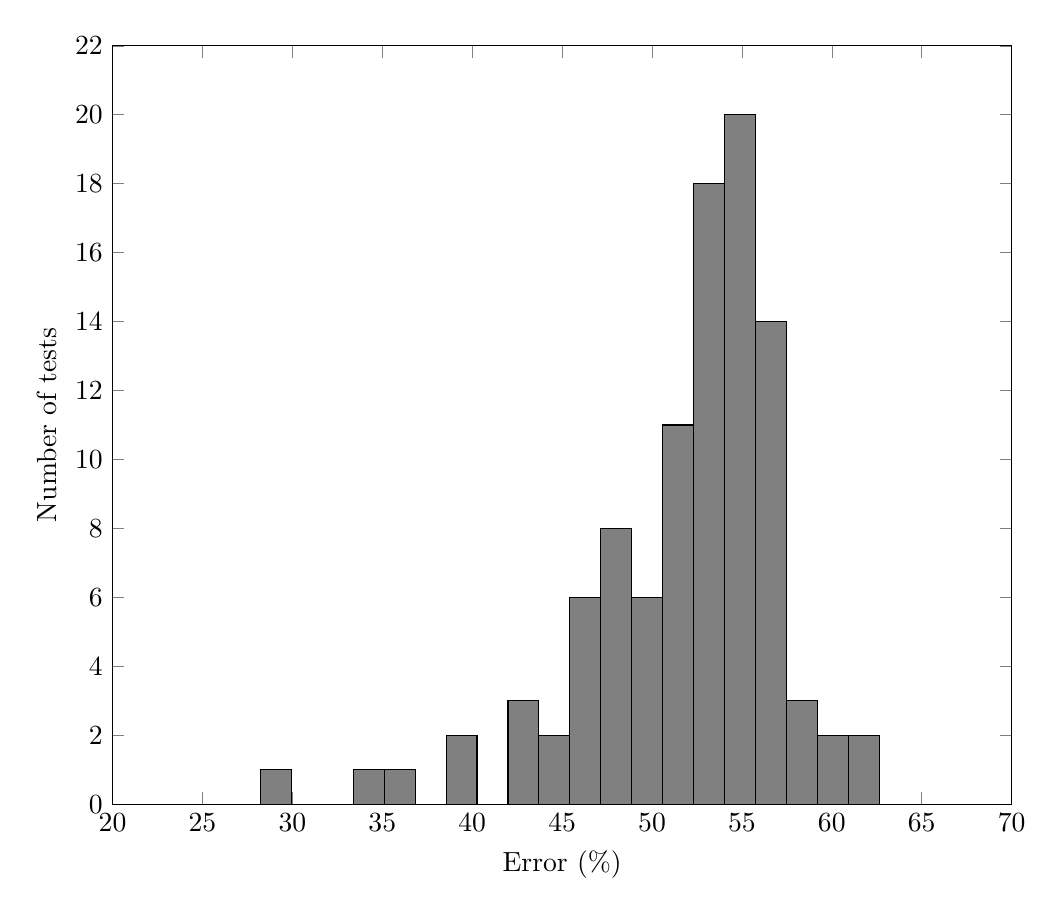
\begin{tikzpicture}
  \begin{axis}[
    width=13cm,
    ylabel=Number of tests,
    xlabel=Error (\%),
    xmin=20,xmax=70,ymin=0,]
    \addplot [ybar interval,fill=gray,draw=black] coordinates {
(28.22526783,  1.)
(29.94580833,  0.)
(31.66634883,  0.)
(33.38688933,  1.)
(35.10742983,  1.)
(36.82797033,  0.)
(38.54851083,  2.)
(40.26905133,  0.)
(41.98959183,  3.)
(43.71013233,  2.)
(45.43067283,  6.)
(47.15121333,  8.)
(48.87175383,  6.)
(50.59229433, 11.)
(52.31283483, 18.)
(54.03337533, 20.)
(55.75391583, 14.)
(57.47445633,  3.)
(59.19499683,  2.)
(60.91553733,  2.)
(62.63607783,  0.)
    };
  \end{axis}
\end{tikzpicture}